\section{UI design}

As we describe in figure ~\ref{fig:mainui}, Our UI has four main parts: the search bar, scatterplots for word vectors, statistics for SNLI task and sentences for selected word.

Also we put interactive functions to the scatterplots, People can click or brush a rectangle to select points in them, poeple can also zoom in/out the plots. For plot in the right-hand side, people can change the color from gold label to predicted label, they can also change the color based on the prediction correctness(green for positive and red for negative) as shown in figure ~\ref{fig:color} 

For the statistic table, we can click each cell and filter the scatterpolt based on the selection. As shown in figure ~\ref{fig:stat}, we clicked the number of entailments predicted as contradictions.

We can click the sentence and show all words vectors in the scatterplots. We use same color and switch button for sentences as for right plot

\subsection{Observations}

Mainly we observe three interesting facts in this project:

{\flushleft {\bf (1)}}  
We can see that before fine-tuning, the vectors locates in a random place, and for each word, the vectors cluster by its semantic meanings, for example, vectors for dog for hot dog locate in a different cluster from dog for animals.

{\flushleft {\bf (2)}} 
After fine-tuning, the vectors are clustered by the task label and lose its semantic information which we believe it is kind of overfeeding because even the task-free tokens like . or [SEP] are also clustered based on the task.

{\flushleft {\bf (3)}} 
Although we don't feed any information to our model about the meaning of entailment, contradiction and neutral, fine-tuned BERT somehow learn that neutral is a status between entailment and contradiction.

\begin{figure*}[h]

\centering
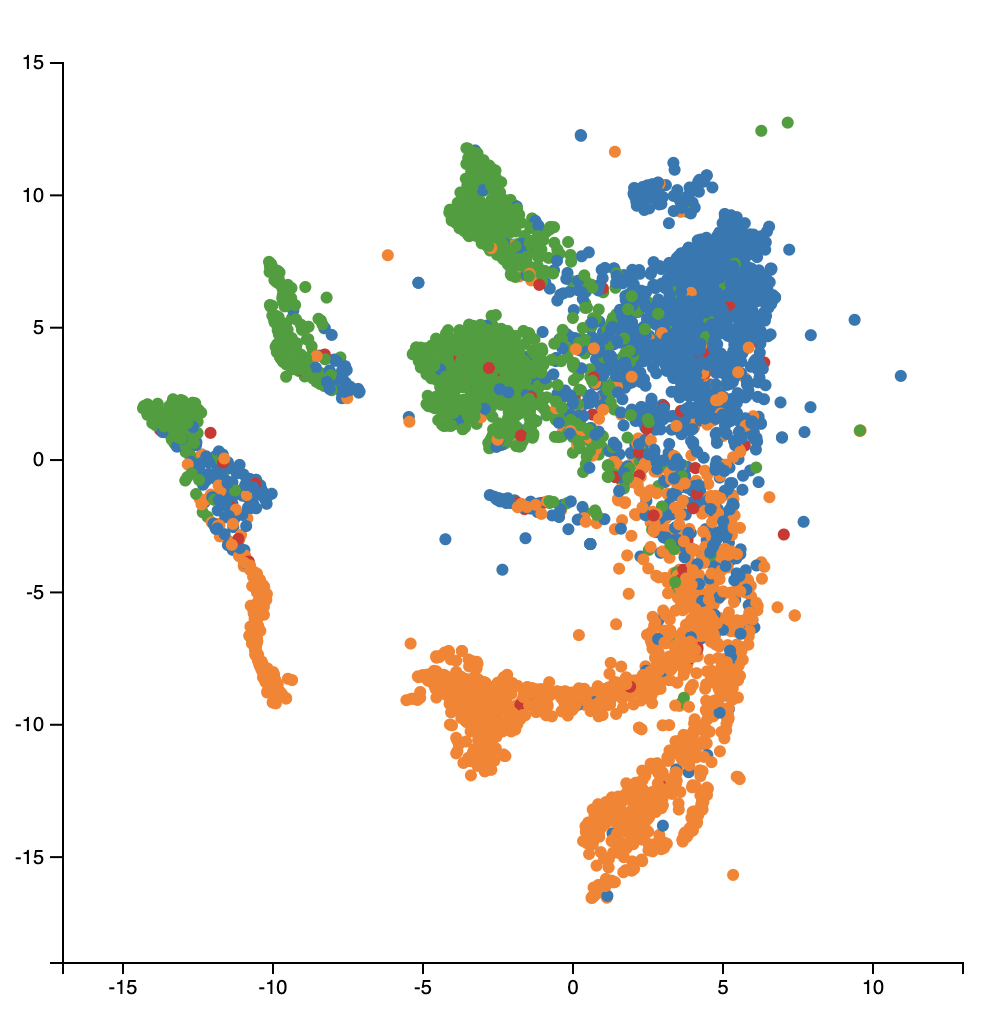
\includegraphics[width=.3\textwidth]{figs/fig2.png}\hfill
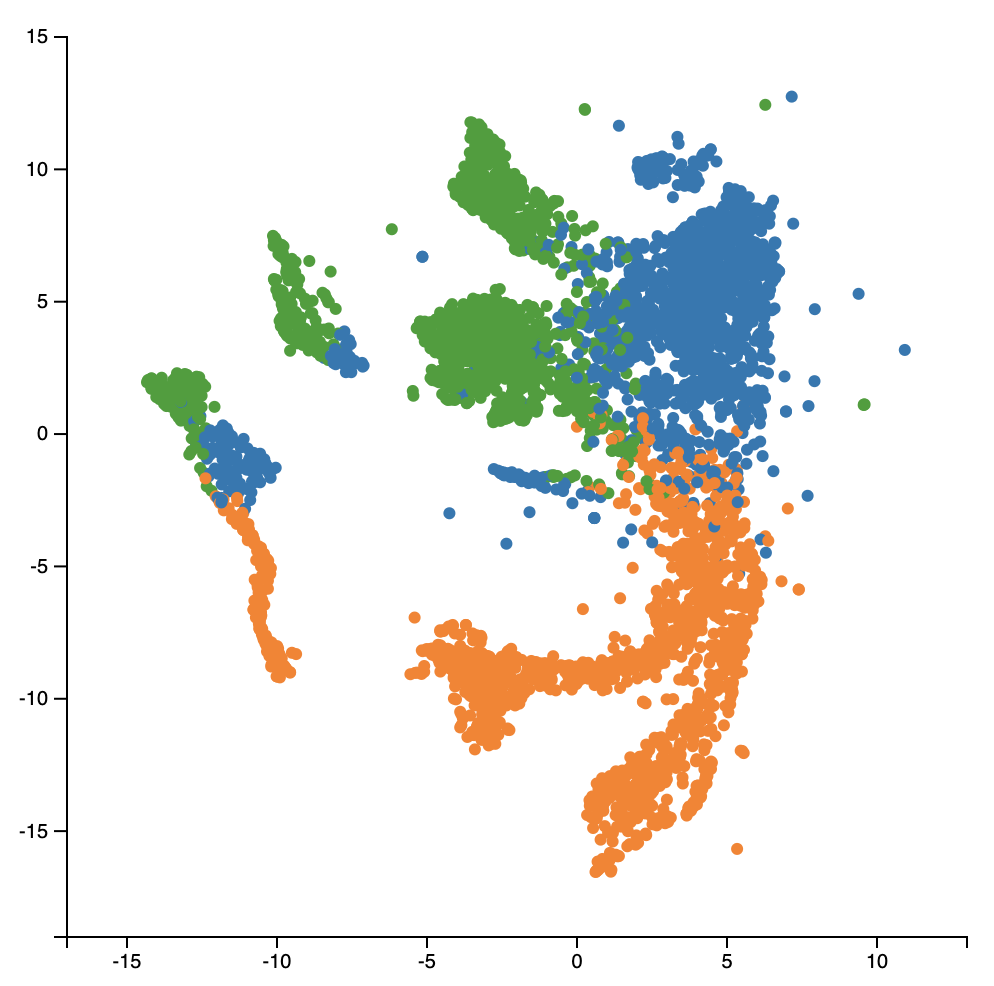
\includegraphics[width=.3\textwidth]{figs/fig3.png}\hfill
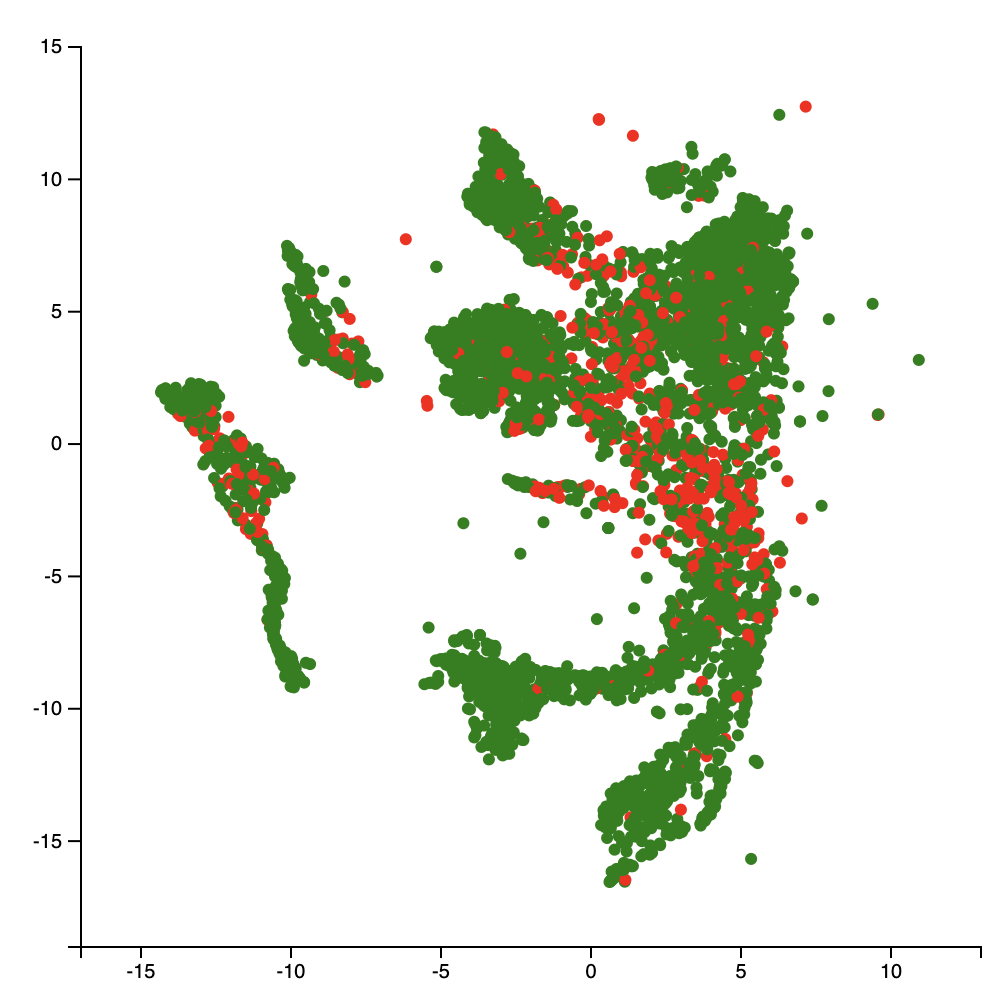
\includegraphics[width=.3\textwidth]{figs/fig4.png}

\caption{scatterplot color changing}
\label{fig:color}

\end{figure*}

\begin{figure}[b]

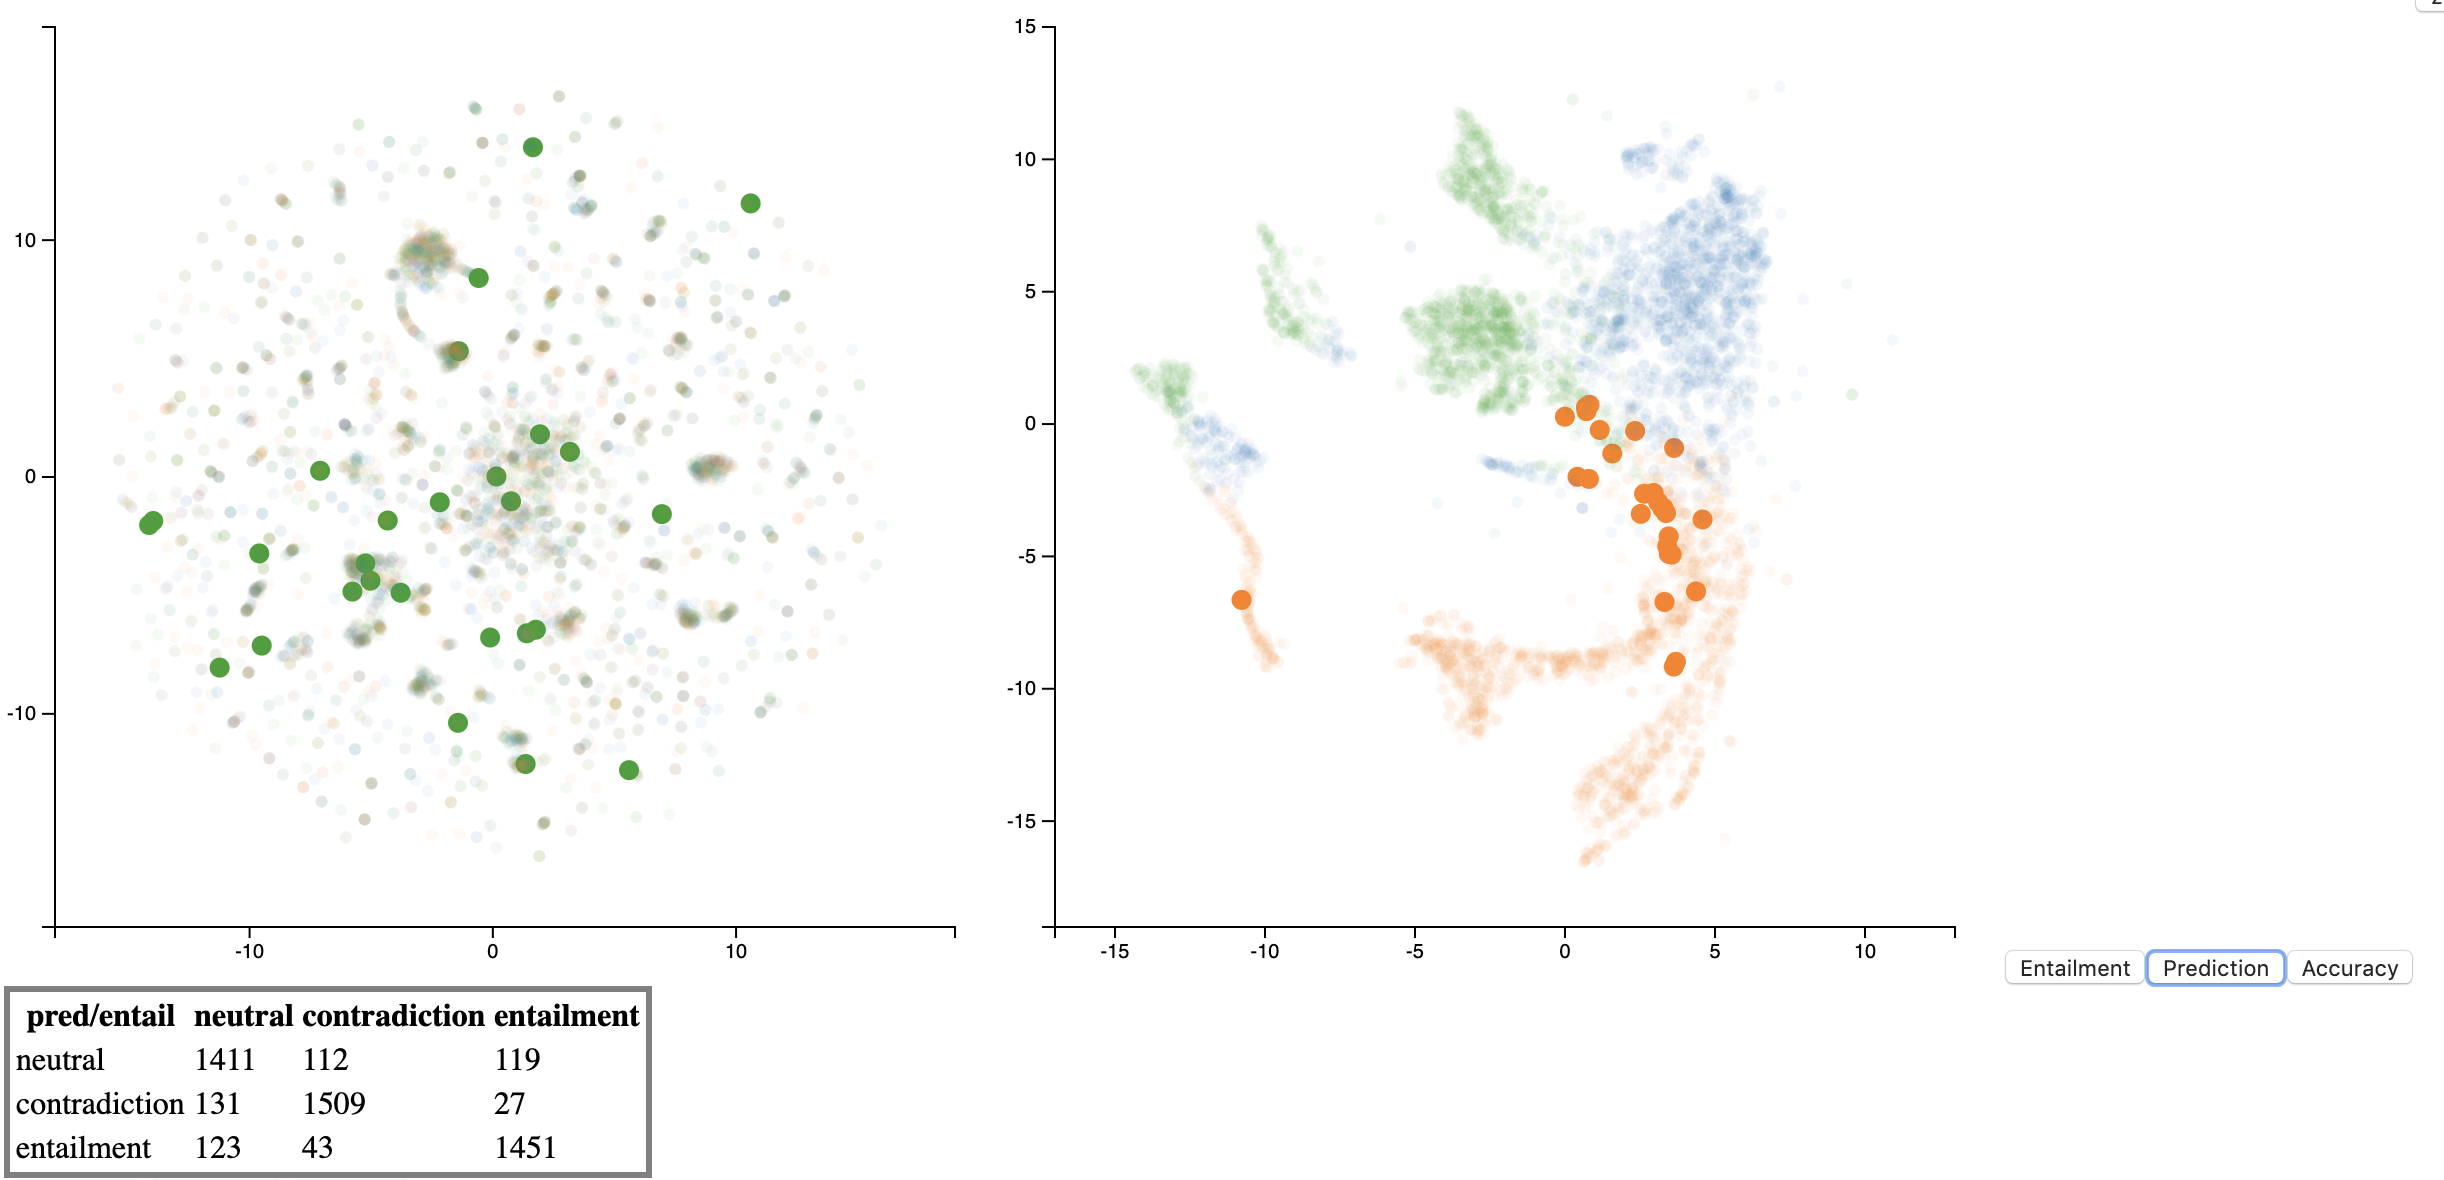
\includegraphics[width=.45\textwidth]{figs/fig5.png}

\caption{Shown only words in an entailment pair but labeled as contradiction}
\label{fig:stat}

\end{figure}